\subsection{File Cache Size}

\subsubsection{Estimation}

Linux uses all available memory as a file cache, therefore the minimum size
file cache is 0MB if applications and kernel are using the entire memory. With this information we estimate that the maximum size file cache is the 
total size of memory minus the size of the linux kernel. To estimate the size of memory occupied by the kernel we clear the file cache by executing 
the following command:
\begin{verbatim}
echo 3 > /proc/sys/vm/drop_caches
\end{verbatim}
and then running the free program to report memory usage statistics. This shows that 4GB out of 8GB in memory are available to be used as a file cache.

\subsubsection{Methodology}

We implement a program that reads files of varying sizes and reports the read bandwith. For smaller file
sizes we expect the bandwidth to be high. Once the size of the file exceeds the size of the file cache,
we expect to see a drop in read performance. The file size at which read bandwidth drops should 
correspond with the file cache size.

The program obtains a file descriptor to the raw disk in read only mode with the file cache enabled. 
We read from the file descriptor one MB at a time until the desired file size is reached and at that 
point the lseek64() system call is invoked to return the read pointer to the beginning of disk. The process of reading from beginning of disk to the current file size repeats until a timeout signal is asserted.
We begin timing before the first call to read and end timing after a set period of time. We determined 
empirically that 5 seconds is sufficient to perform enough repititions of entire file reads for all 
file sizes tested.

\subsubsection{Results}

Our results are presented in figure~\ref{figure:cacheresult}.

\begin{figure}
    \centering
    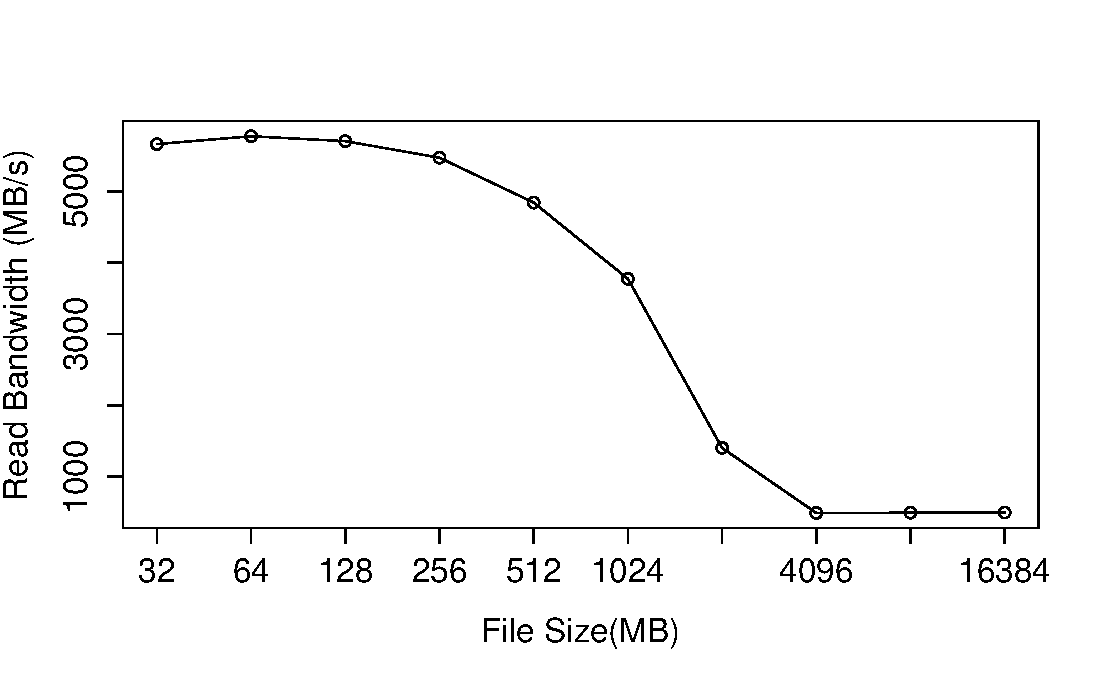
\includegraphics[width=0.5\textwidth]{cache-results.pdf}
    \caption{Experimental results for file cache size}
    \label{figure:cacheresult}
\end{figure}

\subsubsection{Analysis}

The results of our experiment show that for file read bandwidth exceeds the rated maximum bandwidth of the SSD (500MB/s) for file sizes greater than 4GB. This indicates that no file reads are cached because 
the file size is at least twice as large as the cache. According to our results we have over estimated the size of our file cache. The true size of the file cache appears to be between 512MB and 2GB where we 
see a corresponding decrease in the read bandwidth. 

\subsection{File Read Time}

In this section, we describe the time taken to read a file sequentially or randomly.

\subsubsection{Estimation}

Sequential access of a file is when we get the most out of the disk bandwidth. According to our vendor's specification, the maximum read throughput is 520MB/s. We are using a trick : we are not reading off a file that we have created. Rather, we are reading directly of from a disk partition, using a special file : \texttt{/dev/sda1}. In linux systems, \texttt{/dev/sda[x]} is the name of the special file representing disk partition \texttt{x}. There is no reason for a disk partition to be scattered across the disk (the way a user-generated file could be), therefore we can expect our disk access to be almost truly sequential (we still might have to fetch metadata on some other partition). As seen in class, we expect random access to be a lot slow than sequential access when accessing a file through disk. However, our machine uses a SSD, which are known to have much better seek times than traditional hard drives. 

\subsubsection{Methodology}

In order to ensure we are reading from disk and not from the file cache, we use the Linux flag \texttt{O\_DIRECT}. The \texttt{O\_DIRECT} flag can be specified when making the \texttt{open} system call. If used, it guarantees all read and write system calls on the opened file descriptor will fetch data from disk. We read from the \texttt{/dev/sda1} disk one MB at a time in a simple loop. We simulate different file sizes by setting a limit on the loop (called \texttt{total\_size}). When we reach the end of the loop we seek back to the beginning of the loop as follows : 

\begin{lstlisting}
if (total_read >= total_size) {
  retval = lseek64
     (fd, 0, SEEK_SET);
  total_read = 0;
  //...
\end{lstlisting}

where \texttt{total\_read} is the number of blocks read up to now in this iteration. To read blocks randomly, we also read directly from the disk partition. We use the \texttt{lseek} command which reads at an offset of a file descriptor, as follows:

\begin{lstlisting}
numblocks = SIZE_OF_FILE;
offset = (off64_t) numblocks *
  rand() / RAND_MAX;
retval = lseek64(fd, BLOCKSIZE 
  * offset, SEEK_SET);
\end{lstlisting}

where fd is the file seeked (in our case the disk partition), offset is the randomly chosen offset. \texttt{SEEK\_SET} is an option which tells the \texttt{lseek} command to start offsetting from the beginning of the file. Finally, we simulate files of varying size by changing the \texttt{numblocks} variable. To obtain the block size, we used a system command, \texttt{blockdev --getbsz /dev/sda1}; we found it was 4096. Notice we try to maximize bandwidth while reading truly randomly by seeking after each block read. If we read more than one block, than our read pattern would be partly sequential. If we read less, than we would not maximize our read bandwidth. Finally, in order to have good enough simulation we iterate continuously for 10 seconds and then measure the average time it takes to read one block into memory per millisecond.

\subsubsection{Results}

\begin{figure*}
 \centering
  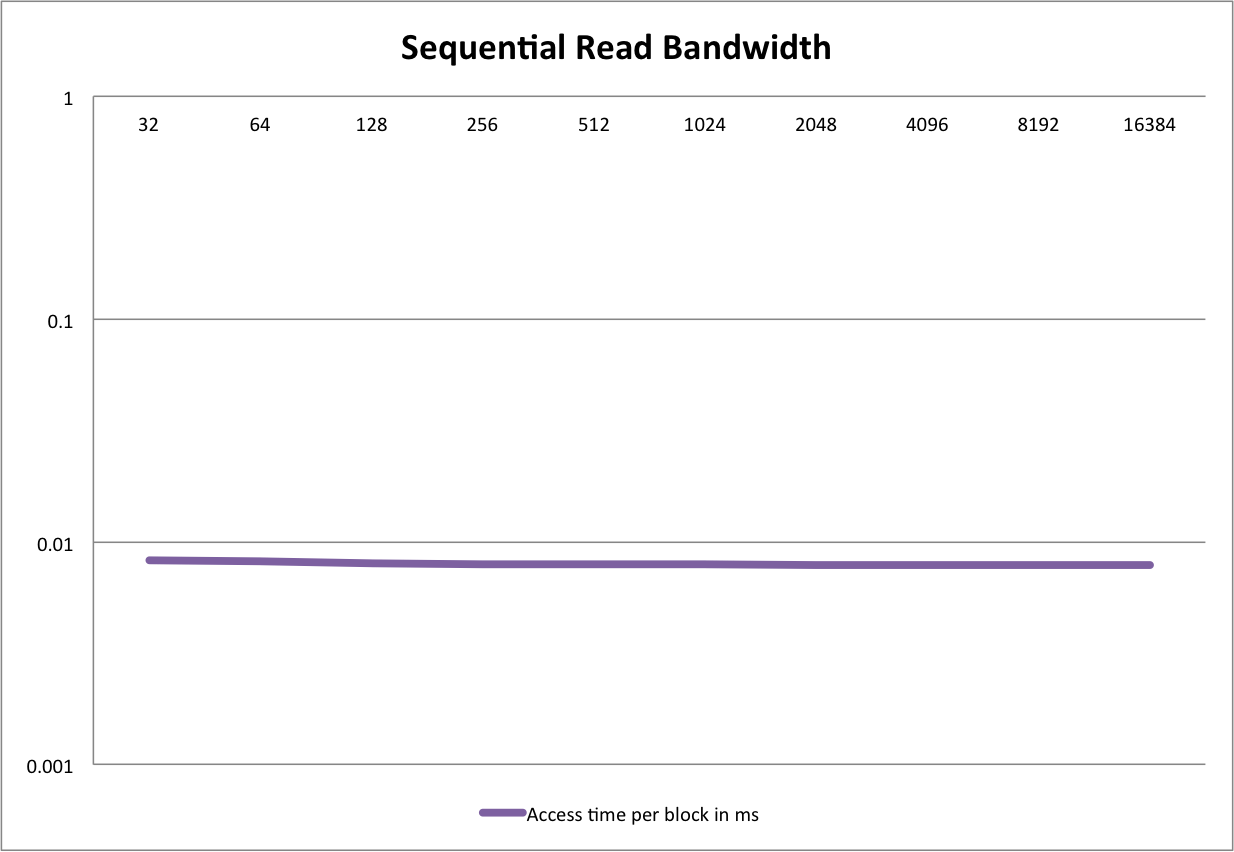
\includegraphics[width=0.85\textwidth]{image/sequential_read.png}
  \caption{Sequential Access Bandwidth}
 \label{fig:sequential}
\end{figure*}

\begin{figure*}
 \centering
  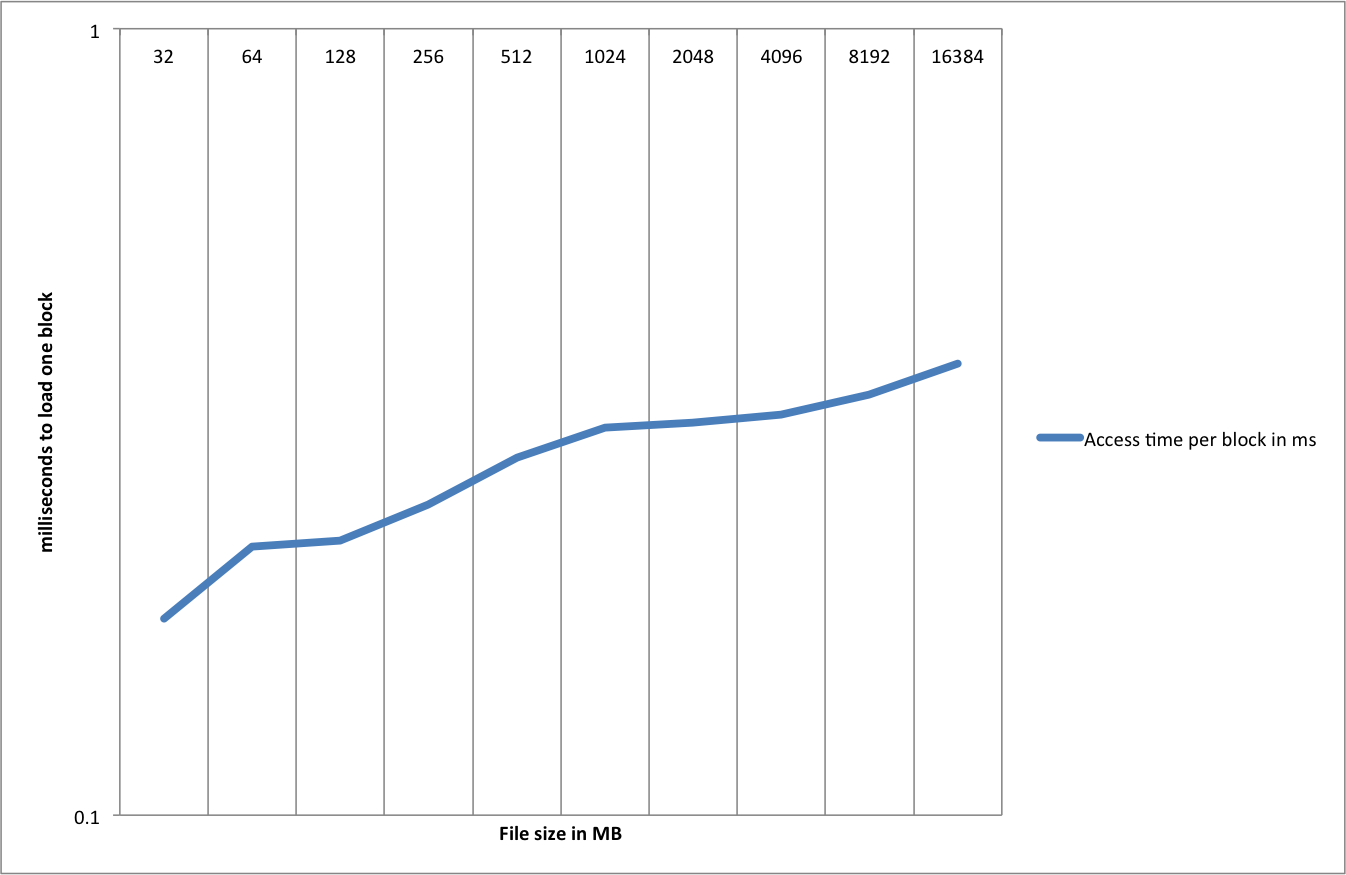
\includegraphics[width=0.85\textwidth]{image/random_read.png}
  \caption{Random Access Bandwidth}
 \label{fig:random}
\end{figure*}

\subsubsection{Analysis}

\subsection{Remote File Read Time}

\subsubsection{Estimation}

Our experiments used an exported file shared from an NFS version 3 server. NFS
version 3 uses TCP by default for data transport.  We estimate that the file
read bandwidth over NFS will be limited by the maximum throughput of the TCP
protocol. We will use the result from our peak bandwidth experiment to estimate 
that the file read bandwidth over NFS will be 16Mbps.

\subsubsection{Methodology}

We configure an NFS server on the same remote machine that was used in the Network bencmarking experiments and share a directory containing a 5GB file. The nfs share is mounted on our local machine and a 
modified version of the random access bandwidth experiment is performed. We modify the program for measuring the read bandwidth of random accesses so that O\_DIRECT flag is not used. This was required because 
it is not supported for reading NFS shares. Random access was chosen over sequential reads in order to limit the effect of the file cache upon our results.

\subsubsection{Results}

Our program outputs the results in MB per second as show in figure~\ref{figure:nsfresult}.

\begin{figure}
    \centering
    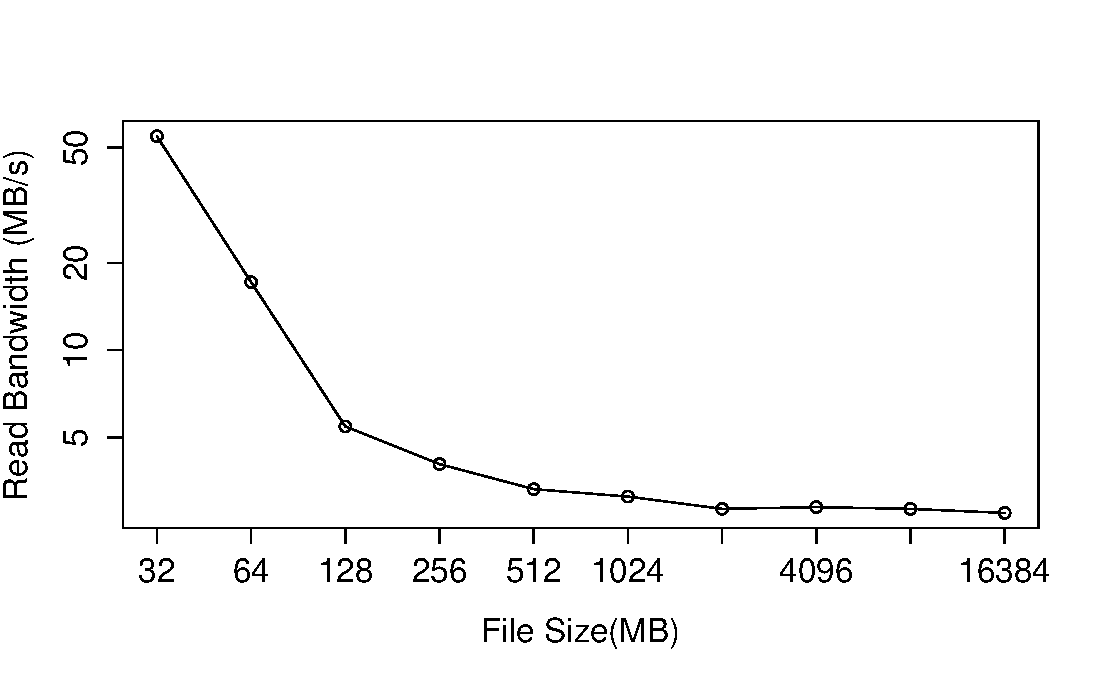
\includegraphics[width=0.5\textwidth]{nfsresults.pdf}
    \caption{log-log plot of experimental results for NFS read bandwidth}
    \label{figure:nfsresult}
\end{figure}

\subsubsection{Analysis}

The results show that read bandwidth is greater than our estimate for small
file sizes. This is due to data being accessed from the file cache.  The
experiment is run over the same period of time for each file size, therefore
smaller file sizes will have more opportunities for cache hits with random
access reads than larger file sizes because the overall working set is smaller.
The data shows that as file size increases, the read bandwidth approaches our
estimate that was based upon our previous experimental result of peak bandwidth
over TCP. The minimum read bandwidth is 2.7MB/s which is slightly better than
the peak bandwidth of TCP this is the expected result since the file cache was
not disabled due to reading files over NFS.

\subsection{Contention}

\subsubsection{Estimation}

\subsubsection{Methodology}

\subsubsection{Results}

\subsubsection{Results}

\begin{figure*}
 \centering
  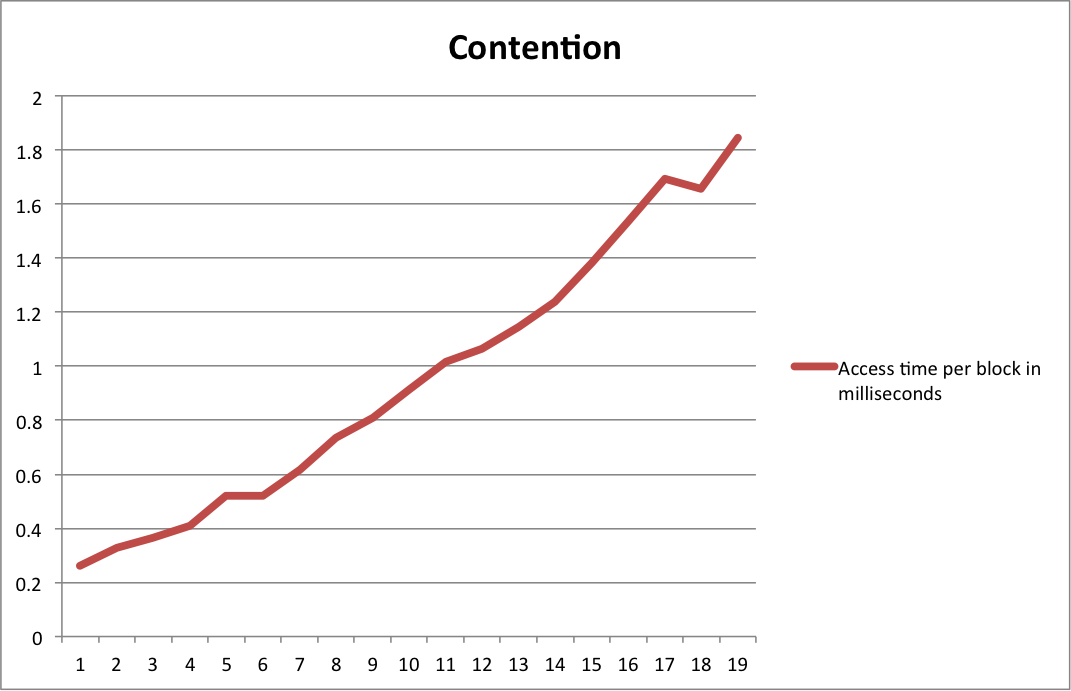
\includegraphics[width=0.85\textwidth]{image/contention.png}
  \caption{Sequential Access Bandwidth}
 \label{fig:contention}
\end{figure*}

\subsubsection{Analysis}
